\section{Antecedentes y justificación}
El objetivo de esta sección es describir las condiciones del marco en el que se
lleva a cabo el proyecto, se recopilarán datos e información sobre la situación
actual en lo que respecta al FJSP, incluyendo la utilización de diferentes
técnicas que han sido utilizadas históricamente para su resolución. Para ello,
se revisará el estado del arte y las últimas tendencias en este campo, con el
fin de obtener una mejor comprensión del problema y explicar la oportunidad de
realizar nuevos aportes en esta área de investigación.

\subsection{Estado del arte}
\subsubsection{Metodos exactos}
Los métodos exactos se basan en la resolución matemática del problema, y pueden
garantizar la obtención de soluciones óptimas en teoría. Sin embargo, estos
métodos suelen ser computacionalmente costosos y, por lo tanto, se aplican
principalmente a problemas de tamaño reducido.\medskip

En el caso del FJSP, algunos métodos exactos que se han utilizado incluyen la
programación lineal de enteros mixta (MILP)\cite{milp}, que modela el problema
como un conjunto de restricciones lineales y una función objetivo lineal, y la
programación por restricciones (CP)\cite{wikiCP}, que reduce el problema a un
conjunto de restricciones lógicas y utiliza técnicas de búsqueda para encontrar
soluciones que satisfagan todas las restricciones. Existen aplicaciones hechas
por Google como Ortools\cite{ortools} o por IBM como CPLEX\cite{cplex}, que son
ejemplos de software que utilizan estos métodos exactos para resolver problemas
de optimización. Estas aplicaciones son muy útiles para resolver instancias de
tamaño reducido, pero no son capaces de resolver instancias de tamaño grande,
debido a la gigantesca a la complejidad que presentan los problemas NP-Hard.

\subsubsection{Metodos heurísticos}
Un método heurístico\cite{Novoseltseva_2021} es un algoritmo o técnica de
búsqueda que está diseñado para encontrar soluciones aproximadas a problemas de
optimización, cuando las soluciones exactas son difíciles de encontrar. Los
métodos heurísticos son útiles cuando el tiempo y los recursos son limitados, y
cuando el problema a resolver es demasiado complejo para ser resuelto por
medios exactos. Los métodos heurísticos pueden ser aplicados a una amplia
variedad de problemas de optimización, incluyendo el FJSP.\medskip

En el caso del FJSP, existen diferentes métodos heurísticos que se han
utilizado con éxito para encontrar soluciones aproximadas. Un ejemplo es el
algoritmo de búsqueda tabú\cite{Howell_2023}, que se basa en la exploración de
soluciones vecinas para encontrar soluciones cada vez mejores. Otro ejemplo es
el algoritmo de búsqueda local, que busca soluciones iterativamente en una
vecindad de soluciones. También se han utilizado enfoques basados en la
construcción de soluciones parciales donde se construyen soluciones en etapas,
utilizando información previa y reglas heurísticas para guiar el proceso de
construcción. Todos estos métodos heurísticos han demostrado ser efectivos para
resolver el problema de FJSP, y se pueden adaptar y mejorar para abordar
variantes más complejas del problema.

\subsubsection{Metodos metaheurísticos}
Una metaheurística\cite{Metaheuristic_2023} es una estrategia general para
resolver problemas de optimización. A diferencia de las heurísticas, las
metaheurísticas no están diseñadas para resolver problemas específicos, sino
que proporcionan un marco flexible y genérico para abordar una amplia gama de
problemas de optimización. Las metaheurísticas son algoritmos de búsqueda
inteligentes que se inspiran en procesos naturales o en conceptos matemáticos
abstractos, y son capaces de explorar y explotar el espacio de soluciones en
busca de soluciones óptimas o de alta calidad.\medskip

Algunos de los enfoques más conocidos son el algoritmo genético, que se inspira
en la evolución biológica, y el enjambre de partículas, que se basa en el
comportamiento de las colonias de organismos sociales. Estos algoritmos
utilizan técnicas como la generación aleatoria de soluciones iniciales y la
exploración sistemática del espacio de búsqueda para encontrar soluciones
óptimas o de alta calidad. La exploración implica buscar soluciones en
diferentes regiones del espacio de soluciones, mientras que la explotación se
refiere a mejorar las soluciones encontradas para acercarse a la solución
óptima.

\subsubsection{Algoritmos genéticos}
Los algoritmos genéticos\cite{GeneticAlgorithm_2023} son una técnica de
optimización inspirada en la evolución biológica. Estos algoritmos imitan el
proceso de selección natural, reproducción y mutación en la búsqueda de
soluciones para problemas de optimización combinatoria. La idea básica de los
algoritmos genéticos es utilizar la selección natural para encontrar soluciones
mejores a través de la generación de nuevas soluciones a partir de las ya
existentes junto a la aplicación de operadores de cruce y mutación.\medskip

En la literatura, estos algoritmos han sido ampliamente utilizados y han
demostrado ser efectivos para encontrar soluciones de alta calidad. La
representación cromosómica utilizada en los algoritmos genéticos se basa en la
codificación de una solución del problema de FJSP como una cadena de genes, y
los operadores genéticos como el cruzo o la mutación, se aplican para producir
nuevas soluciones o realizar ligeros cambios en aquellas ya existentes. Una de
sus principales ventajas es que pueden manejar fácilmente múltiples objetivos y
restricciones adicionales, y son capaces de explorar ampliamente el espacio de
soluciones.\medskip

En cambio uno de sus problemas es que los algoritmos genéticos pueden requerir
una gran cantidad de tiempo y esfuerzo para encontrar soluciones aceptables, y
no siempre garantizan encontrar la mejor solución posible. Además, pueden
requerir ajustes cuidadosos de los parámetros y una cuidadosa selección de
operadores para funcionar bien en diferentes instancias del problema y tienen
tendencia a sufrir de prematura convergencia lo que genera dificultades para
escapar de óptimos locales.

\subsubsection{Redes neuronales}
Las redes neuronales\cite{McNelis_2005} son una clase de algoritmos de
aprendizaje automático inspirados en la estructura y el funcionamiento del
cerebro humano. Estas redes están formadas por múltiples capas de neuronas
interconectadas que procesan información para resolver problemas de
clasificación, regresión, reconocimiento de patrones, entre otros.\medskip

En el contexto del FJSP, las redes neuronales pueden ser utilizadas para
aprender patrones en los datos de entrada del problema, como la secuencia de
tareas y las restricciones de precedencia. Esto puede ayudar a generar
soluciones de alta calidad al FJSP, incluso para instancias de problemas
grandes y complejas. Además, las redes neuronales también pueden ser entrenadas
para mejorar la calidad de las soluciones generadas por otros algoritmos de
optimización, como los algoritmos genéticos y los métodos heurísticos.\medskip

La principal ventaja de las redes neuronales es su capacidad para manejar datos
no lineales y ruidosos, y para detectar patrones complejos en los datos de
entrada. Sin embargo, las redes neuronales también pueden presentar desafíos en
el entrenamiento y ajuste de los hiperparámetros, y pueden ser propensas a
sobreajuste si no se controlan adecuadamente, pero incluso con esos
inconvenientes son una de las técnicas más prometedoras para el FJSP y pueden
ser utilizadas en combinación con otras técnicas de optimización para mejorar
la calidad de las soluciones.

\subsubsection{Redes neuronales de grafos}
Una GNN (Graph Neural Network)\cite{pytorch-geometric} es un tipo de red
neuronal que se utiliza para analizar y procesar datos estructurados en forma
de grafos. A diferencia de los modelos tradicionales que trabajan
principalmente con datos tabulares, las GNN están diseñadas específicamente
para trabajar con datos en los que las relaciones entre los elementos son
fundamentales, como redes sociales, redes de transporte, moléculas, etc. Aunque
no son tan populares como las redes neuronales tradicionales y no hay tantos
estudios sobre su aplicación al FJSP, las GNN son un área de investigación muy
prometedora en este tipo de problemas ya que ofrecen una forma natural de
representar las restricciones y relaciones entre las tareas y las
máquinas.\medskip

El funcionamiento de una GNN se basa en la propagación de la
información\cite{Message_parrs} a través de los nodos de un grafo. Cada nodo en
el grafo representa un elemento de datos y está asociado con un vector de
características. La idea principal de una GNN es que cada nodo actualiza su
vector de características en función de su propio estado actual y la
información de los nodos vecinos. El proceso de propagación de la información
en una GNN generalmente sigue los siguientes pasos:

\begin{itemize}
      \item \textbf{Inicialización:} cada nodo en el grafo se inicializa con un vector de características,
            que puede ser un vector de valores aleatorios o puede estar basado en atributos conocidos del nodo.
      \item \textbf{Agregación:} cada nodo actualiza su vector de características en función de su estado
            actual y la información de los nodos vecinos. La información de los nodos vecinos se agrega utilizando
            una función de agregación, como la suma o el promedio.
      \item \textbf{Actualización:} cada nodo actualiza su vector de características utilizando una función
            de actualización. Esta función de actualización toma como entrada el estado actual del nodo y la
            información agregada de los vecinos, se realiza un procesamiento sobre la red neuronal y se obtiene
            un nuevo vector de características para el nodo.
      \item \textbf{Iteración:} los pasos de agregación y actualización se repiten varias veces hasta que
            se alcanza un estado estable.
      \item \textbf{Salida:} Una vez que se han realizado varias iteraciones, se puede utilizar la información
            actualizada de los nodos para realizar tareas específicas, como clasificación, regresión o predicción de
            enlaces en el grafo.
\end{itemize}

\begin{figure}[ht]
      \centering
      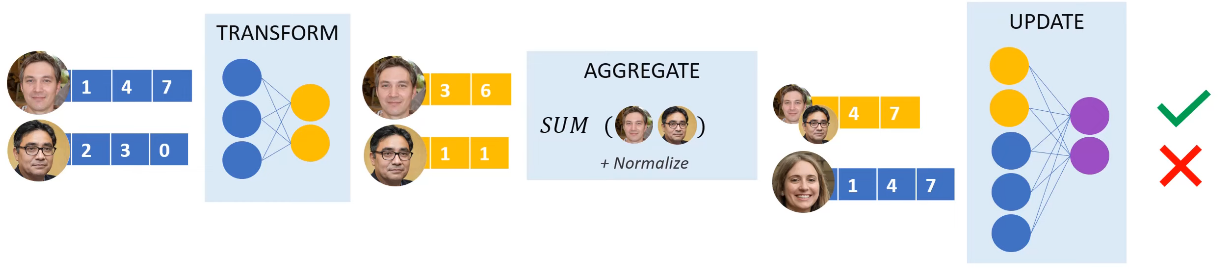
\includegraphics[scale=0.30]{gnnedge.png}
      \caption{Proceso general de propagación de información en una GNN\cite{DeepFindr_2021}.}\label{fig:gnn-edge}
\end{figure}

\subsubsection{Reinforcement learning}
El Reinforcement learning\cite{Bhatt_2018}\cite{Huggingface_DeepRL} es una
técnica de aprendizaje que se basa en la idea de que un agente interactúa con
un entorno para aprender a tomar decisiones óptimas en función de las
recompensa recibida por sus acciones. En el aprendizaje por refuerzo, el agente
aprende a través de la experiencia, probando diferentes acciones y observando
las recompensas asociadas con cada una de ellas, con el objetivo de maximizar
la recompensa total a largo plazo.\medskip

En el contexto del FJSP, el aprendizaje por refuerzo puede ser utilizado para
entrenar a un agente que toma decisiones secuenciales sobre la asignación de
tareas a máquinas y la planificación de la secuencia de tareas, con el objetivo
de minimizar el tiempo total de producción. Una de las principales ventajas del
aprendizaje por refuerzo es su capacidad para aprender directamente de la
experiencia, sin la necesidad de un modelo matemático explícito del problema,
lo que lo hace útil para resolver problemas complejos como el FJSP u otros. Sin
embargo, el aprendizaje por refuerzo también presenta desafíos en la definición
de la función de recompensa y en la selección de la política óptima que
maximiza la misma. Además, requiere de una gran cantidad de tiempo y recursos
computacionales para entrenar al agente en instancias del problema de FJSP
grandes y complejas. Existen pocos estudios que utilizan el aprendizaje por
refuerzo para resolver el FJSP, pero los resultados obtenidos son prometedores.

\subsubsection{Imitation learning}
El IL\cite{SmartLab_2019} una técnica de aprendizaje en la que un modelo aprende a partir de 
ejemplos proporcionados por un experto. En el IL, el modelo trata de imitar 
la forma en que el experto realiza una determinada tarea, utilizando los 
ejemplos como guía. Además, el experto no tiene por qué ser una persona física, 
también es posible utilizar algoritmos de optimización para generar soluciones 
de alta calidad, y luego utilizar estas soluciones como ejemplos de entrenamiento 
para el aprendizaje.\medskip

Esta técnica puede ser utilizada para aprender a generar soluciones de alta
calidad a partir de configuraciones previamente resueltas por un experto, esto
es gracias a que el modelo es capaz de identificar patrones y características
comunes en las soluciones óptimas del problema. Luego, el modelo puede ser
utilizado para generar nuevas soluciones que imiten el comportamiento del
experto humano. Una de las principales ventajas del aprendizaje por imitación
es que los datos que se le ofrece son soluciones de alta calidad, lo que
agiliza el entrenamiento sin requerir la optimización iterativa del problema.

\subsubsection{Ensemble learning}
Un Ensemble\cite{Kundu_2023} en machine learning, también conocido como ensemble learning, es
una técnica que combina múltiples modelos de aprendizaje automático para
mejorar la precisión y estabilidad de las predicciones. Cada uno de estos
algoritmos puede tener fortalezas y debilidades en términos de su capacidad
para encontrar soluciones óptimas en diferentes instancias del problema. Al
combinarlos en un Ensemble, se pueden aprovechar las fortalezas de cada uno de
ellos y obtener soluciones más robustas y de mejor calidad.\medskip

Cada modelo produce una predicción diferente y las predicciones de los
distintos modelos se combinan para obtener una única predicción. Existen
diferentes tipos de Ensemble como el de por votación, bagging, boosting y
tacking\cite{Ensemble_Algorithms}. Cada uno de estos ensemble representa una 
estrategia diferente para combinar las predicciones de los distintos modelos, 
por ejemplo en el ensamble por votación, cada modelo vota por la acción a la 
que predice, y la resultante con mayor número de votos es la predicción final.

\subsection{Antecedentes}
Una vez terminada la investigación sobre el estado actual del problema, se
explorarán diversas ideas y reflexiones que han supuesto un impacto previo para
la motivación de este trabajo. A nivel de industria, se presentan dos
principales desafíos que enfrenta este problema de optimización combinatoria:
la utilidad de los algoritmos metaheurísticos en escenarios online, y la
capacidad de los usuarios para expresar claramente las funcionalidades y
restricciones del problema. En ambos casos, se explicaran los antecedentes que
han motivado el desarrollo de este trabajo y se presentarán las principales
ideas que se han explorado en la literatura.\medskip

De acuerdo a la investigación realizada con anterioridad, si bien los
metaheurísticos son ampliamente utilizados en la solución de problemas de
optimización, su velocidad y practicidad en situaciones reales pueden ser
limitadas, ya que a menudo requieren de una gran cantidad de iteraciones y
evaluaciones para encontrar una solución óptima. Esto puede resultar en un
tiempo de ejecución prolongado, lo que no es adecuado para aplicaciones en
tiempo real o decisiones a corto plazo. Además, otro de los problemas que
enfrentan los metaheurísticos es su nula reusabilidad de información, ya que
cada vez que se ejecuta el algoritmo, se debe reiniciar desde cero. El buscar
un sistema que pueda resolver el problema en tiempo real es un desafío
importante para la industria, ya que la capacidad de tomar decisiones rápidas y
eficientes es crucial.\medskip

Otro de los desafíos que enfrenta la industria es la capacidad de los usuarios
para expresar claramente las funcionalidades y restricciones del problema. En
la mayoría de las situaciones, los usuarios no tienen conocimientos suficientes
o la capacidad de expresar las restricciones del problema de forma precisa,
pero si son capaces de identificar las soluciones óptimas. Por ejemplo, en el
caso de la logística en el transporte, donde una empresa de transporte de
mercancías puede tener una idea clara de cómo quisiera asignar los vehículos a
las rutas de entrega para minimizar los tiempos de viaje y los costos de
combustible. Sin embargo, expresar todas las restricciones y consideraciones
relacionadas con la capacidad de los vehículos, los horarios de los
conductores, las restricciones de tiempo y las regulaciones de tráfico en una
formulación matemática puede resultar complicado y requerir un conocimiento
técnico multidisciplinario.\medskip

En este escenario, los operadores con experiencia podrían proporcionar
soluciones de alta calidad, que luego podrían ser utilizados como datos de
entrenamiento para un modelo de Deep learning. El modelo aprendería a imitar el
comportamiento del experto a partir de estos ejemplos, capturando así la
intuición y el conocimiento tácito que tienen los usuarios, pero que pueden
tener dificultades para expresar de manera formal. De esta manera, se podrá
abordar la brecha entre el conocimiento tácito de los operadores y la
representación formal de las funcionalidades y restricciones del problema,
permitiendo desarrollar soluciones más precisas y efectivas.\medskip

En conclusión, la idea de aprovechar el conocimiento tácito de los expertos en
la resolución de problemas de optimización combinatoria a través de técnicas de
inteligencia artificial ofrece un prometedor potencial. La capacidad de
capturar el conocimiento de los usuarios que enfrentan dificultades en la
formulación del problema, puede ser clave para mejorar la efectividad en la
toma de decisiones para procesos complejos. Además, si gracias a estas técnicas
logramos inferir una estrategia para construir soluciones a partir de ese
conocimiento, podríamos solucionar colateralmente el problema del tiempo de
ejecución que habíamos identificado en los algoritmos metaheurísticos, ya que
no necesitaríamos explorar todo el espacio de soluciones para encontrar una
solución óptima, lo que nos permitiría reducir el tiempo de ejecución de los
algoritmos drásticamente.

\pagebreak